\documentclass{classrep}
\usepackage[utf8]{inputenc}
\usepackage[pdftex]{graphicx}
\usepackage[polish]{babel}
\usepackage{algorithm}
\usepackage{algorithmic}
\usepackage{multicol}
\usepackage{amsmath}
\usepackage{listings}
\usepackage{array}
\usepackage{multirow}
\usepackage{hyperref}
\usepackage{subfigure}

\studycycle{Informatyka, studia dzienne, II st.}
\coursesemester{I}

\coursename{Metody Obliczeniowe Optymalizacji}
\courseyear{2010/2011}

\courseteacher{mgr inż. Łukasz Chomątek}
\coursegroup{czwartek, 14:15}
\svnurl{https://serce.ics.p.lodz.pl/svn/labs/moo/lcjp_cz1415/wacjan/Zadanie3@118}

\author{%
  \studentinfo{Michał Janiszewski}{169485} \and
  \studentinfo{Leszek Wach}{169513}
}

\title{Zadanie 3: Metoda quasi-Newtona w wersji DFP}

\floatname{algorithm}{Algorytm}

\begin{document}

\maketitle

\section{Cel zadania}
Celem zadania było napisanie programu przeprowadzającego minimalizację funkcji dwóch zmiennych według algorytmu Davidon-Fletcher-Powell.

\section{Metoda rozwiązania}
Metoda Davidona-Fletchera-Powella jest również nazywana metodą przemiennej metryki. Należy do grupy procedur kwazi-newtonowskich, w których kolejne kroki wyliczane są ze wzoru:
\begin{center}
	$z_{i+1} = z_i + \tau_i d_i$
\end{center}
gdzie $d_i = -D_i \nabla f(z_i)$
$D_i$ jest macierzą obliczaną ze wzoru:
\begin{center}
\label{eq.dMatrix}
$D_{i+1} = D_i + \frac{p_i p^{t}_i}{p^{t}_i q_i} - \frac{D_i q_i q^{t}_i D_i}{q^{t}_i D_i q_i}$\\
\end{center}
gdzie $p_i = z_{i + 1} - x_i$ oraz $q_i = \nabla f(z_{i+1}) - \nabla f(z_i)$.

Wartość $\tau$ jest dobierana w każdym kroku tak, aby wartość $f(z_i + \tau_i d_i)$ była najmnijesza. Stosuje się w tym przypadku np. metodę złotego podziału, zauwżyliśmy jednak, że do poprawnego działania tej metody konieczne jest wyznaczenie przedziałów unimodalności funkcji, co odbywa się przez próbkowanie. Wykonaliśmy najpierw próbkowanie, pominęliśmy jednak metodę złotego podziału, gdyż uznaliśmy, że wartości pochodzące z próbkowania w zupełności wystarczą, ponieważ metoda ,,wyższego rzędu'', tj. DFP, i tak poda wystarczająco dobre, jeśli nie lepsze, rozwiązanie.

\section{Opis algorytmu}
\begin{enumerate}
  \item \textbf{Etap 1:}
    \begin{enumerate}
      \item ustal dokładność algorytmu $\epsilon$
      \item wybierz punkt startowy $x_o$
      \item ustal startową postać macierzy $D$ jako macierz jednostkową 
      \item podstaw $z_1 = x_0$
      \item podstaw $n = 1$, $s = 1$
    \end{enumerate}
  \item \textbf{Etap 2:}
    \begin{enumerate}
      \item czy $||\nabla f(z_i)|| < \epsilon $ jeśli tak to stop \label{step.start}
      \item podstaw $d_i = -D_i \nabla f(z_s)$
      \item wyznacz $\tau_i$, tak aby $f(z_i + \tau_i d_i)$ było minimalne
      \item podstaw $z_{i+1} = z_i + \tau_i d_i$
      \item oblicz $p_i$, $\nabla f(z_{i + 1})$ oraz $q_i$
      \item wyznacz $D_i$ ze wzoru \ref{eq.dMatrix}
      \item podstaw $i = i + 1$
      \item czy $i \leq N$, jeśli tak to wykonaj krok \ref{step.start}
    \end{enumerate}
  \item \textbf{Etap 3:}
    \begin{enumerate}
      \item wyświetl kolejne przybliżenia rozwiązania $z_x$ dla $x = 0, 1, \ldots, i$
    \end{enumerate}
\end{enumerate}

\section{Wyniki}
Wyniki funkcji testowych porównane zostały z wynikami podawanymi przez WolframAlpha, przy czym wyniki te musiały zostać ,,nakierowane'' tak aby silnik ten znalazł pewne konkretne minima.

\subsection{Funkcja testowa 1}
Wykorzystaliśmy funkcję
\begin{equation}
  z = sin(x) + cos(y)
\end{equation}

Punkt startowy: $(20, 20)$.

Rozwiązanie znalezione przez WolframAlpha\footnote{\url{http://www.wolframalpha.com/input/?i=min\%28sin\%28x\%29+\%2B+cos\%28y\%29\%29\%2C+16+\%3C+x+\%3C+20\%2C+26+\%3C+y+\%3C+30}}: $(17.2787, 28.2743)$, rozwiązanie znalezione programem (16 iteracji): $(17.2787, 28.2743)$.

\begin{figure}
\noindent\makebox[\textwidth]{%
 \subfigure[Widok X-Y]{
  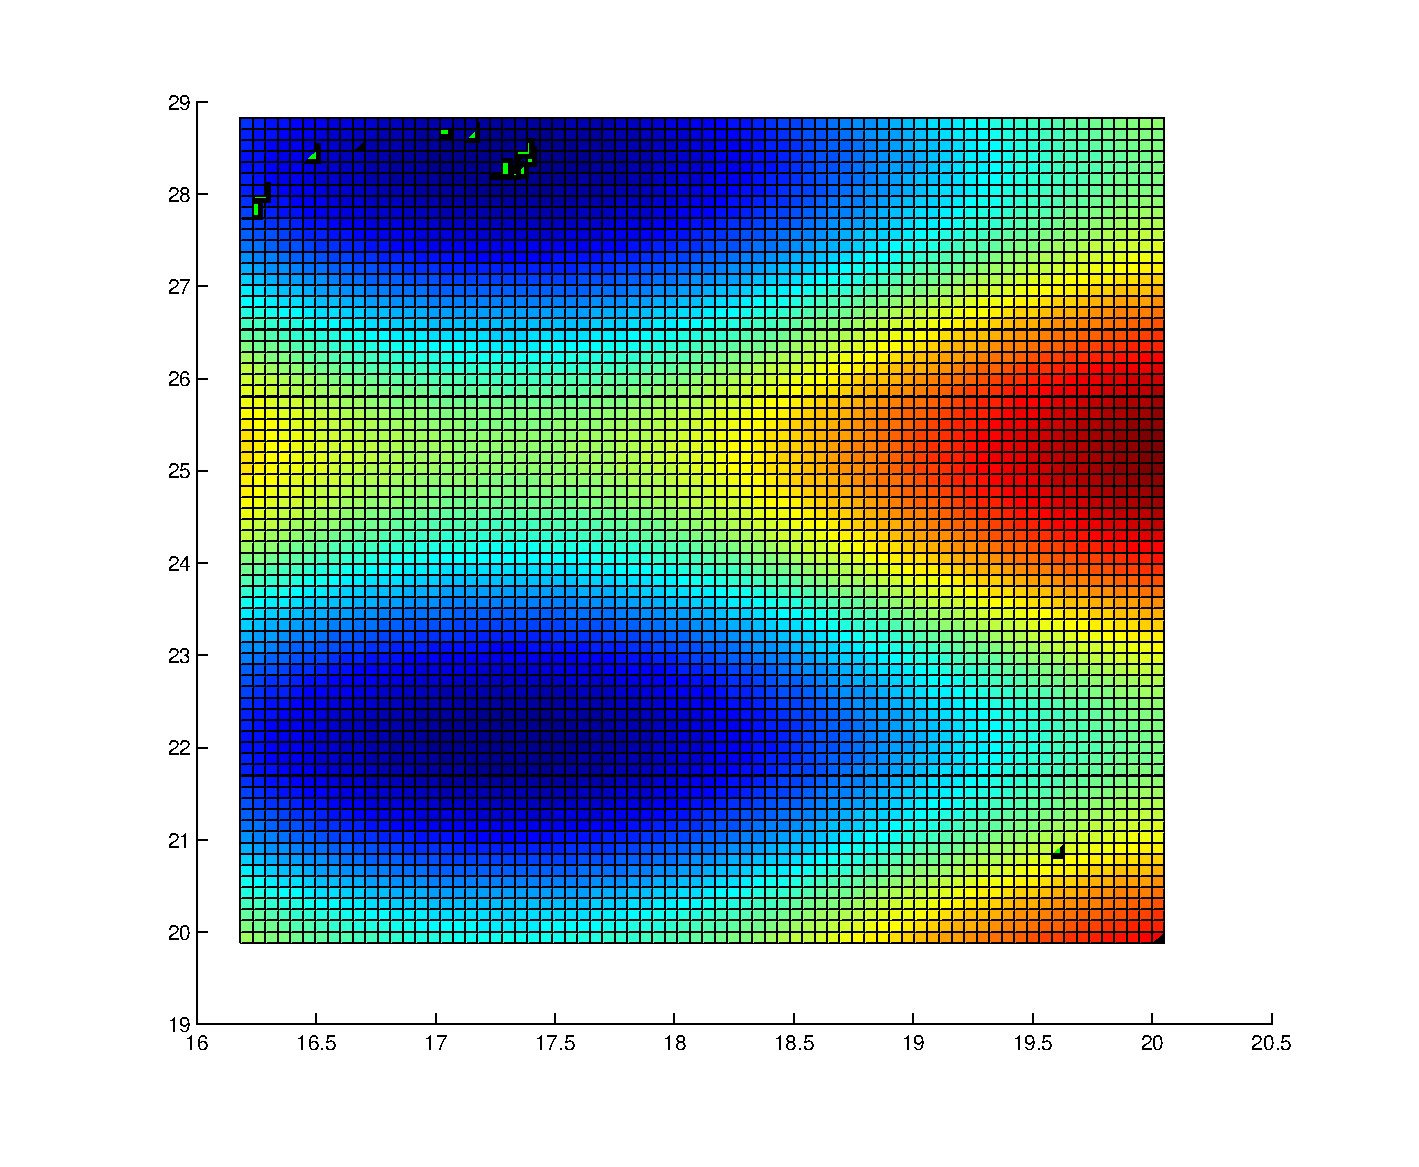
\includegraphics[width=0.5\linewidth]{f1_xy}
 }
 \subfigure[Widok Y-Z]{
  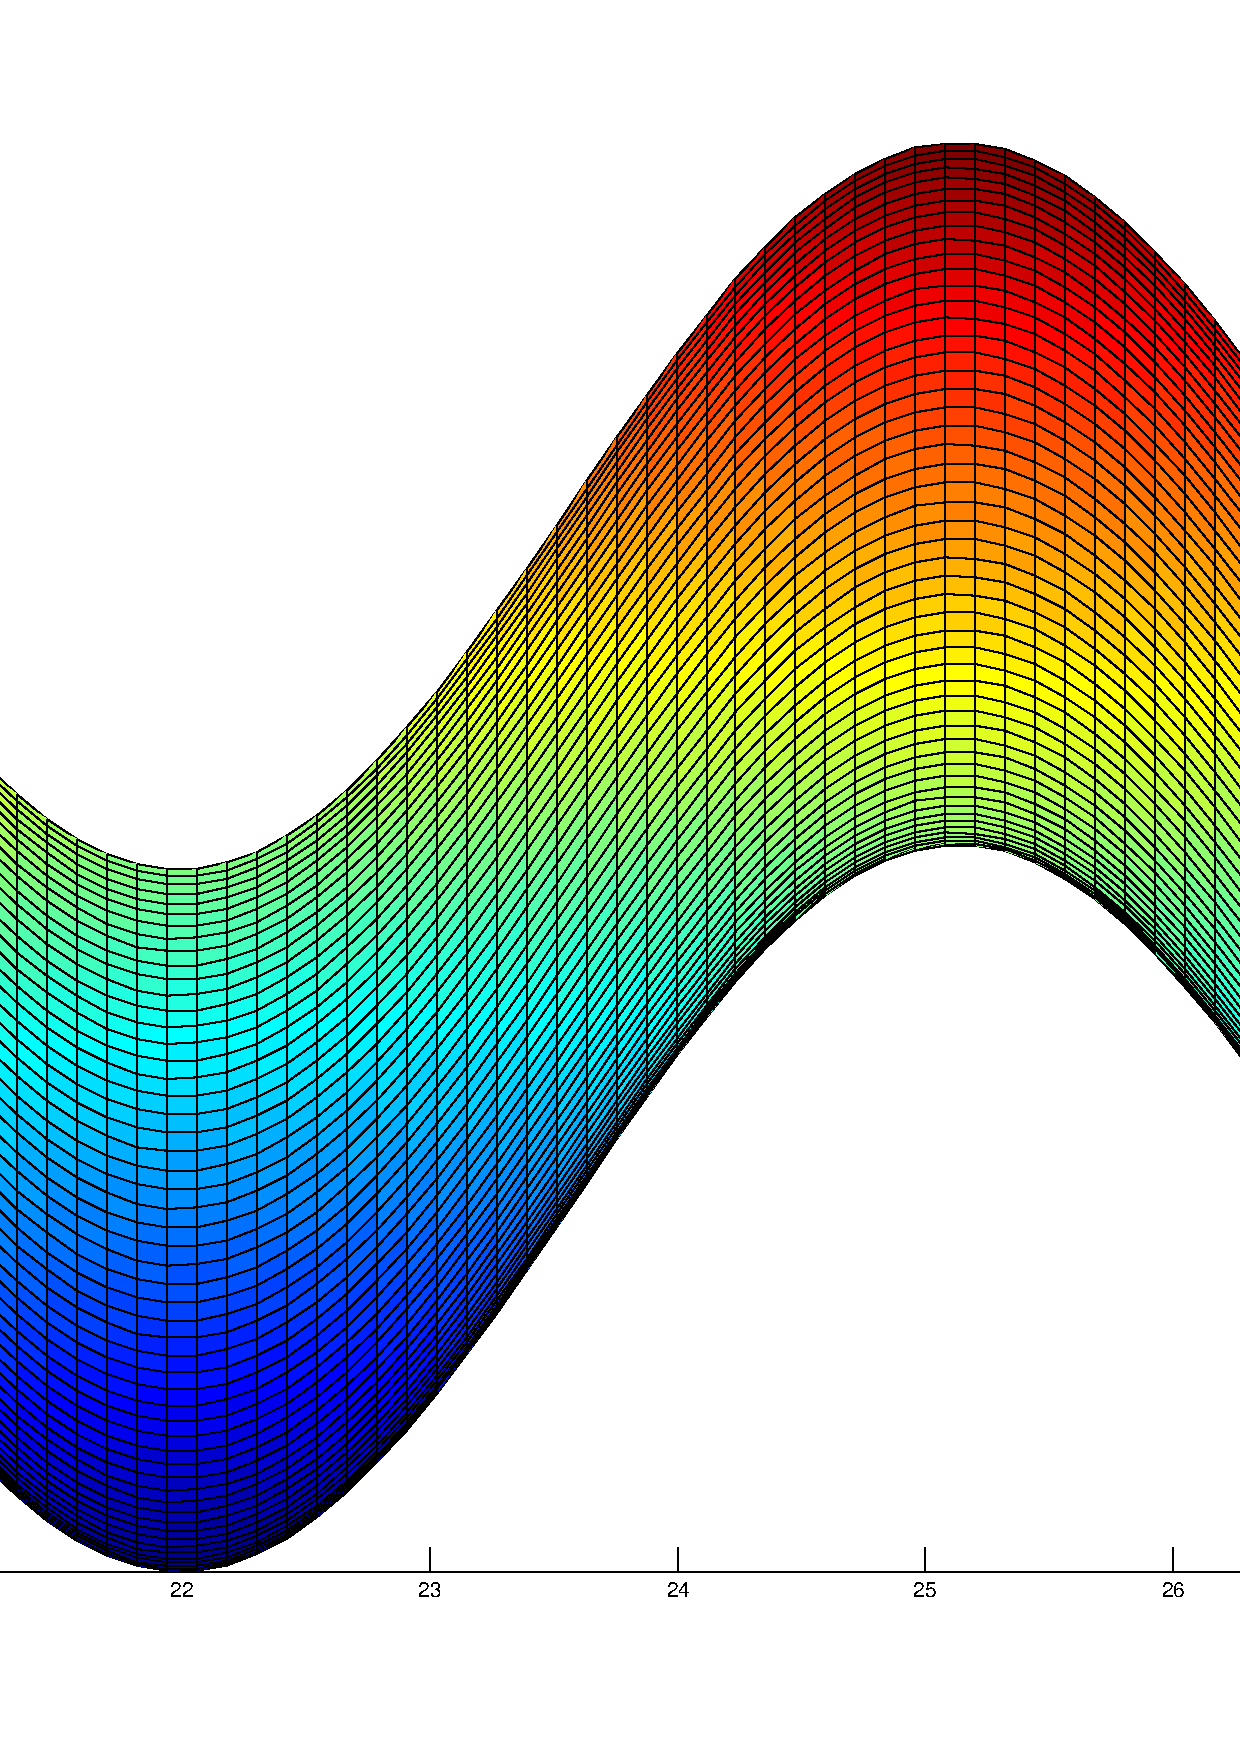
\includegraphics[width=0.5\linewidth]{f1_yz}
 }
}
\caption{Wyniki funkcji 1.}
\end{figure}

\subsection{Funkcja testowa 2}
Wykorzystaliśmy funkcję
\begin{equation}
  z = x^2 + y^2
\end{equation}

Punkt startowy: $(20, 20)$.

Rozwiązanie znalezione przez WolframAlpha\footnote{\url{http://www.wolframalpha.com/input/?i=min\%28x^2+\%2B+y^2\%29}}: $(0, 0)$, rozwiązanie znalezione programem (2 iteracje): $(0, 0)$.

\begin{figure}
\noindent\makebox[\textwidth]{%
 \subfigure[Widok X-Y]{
  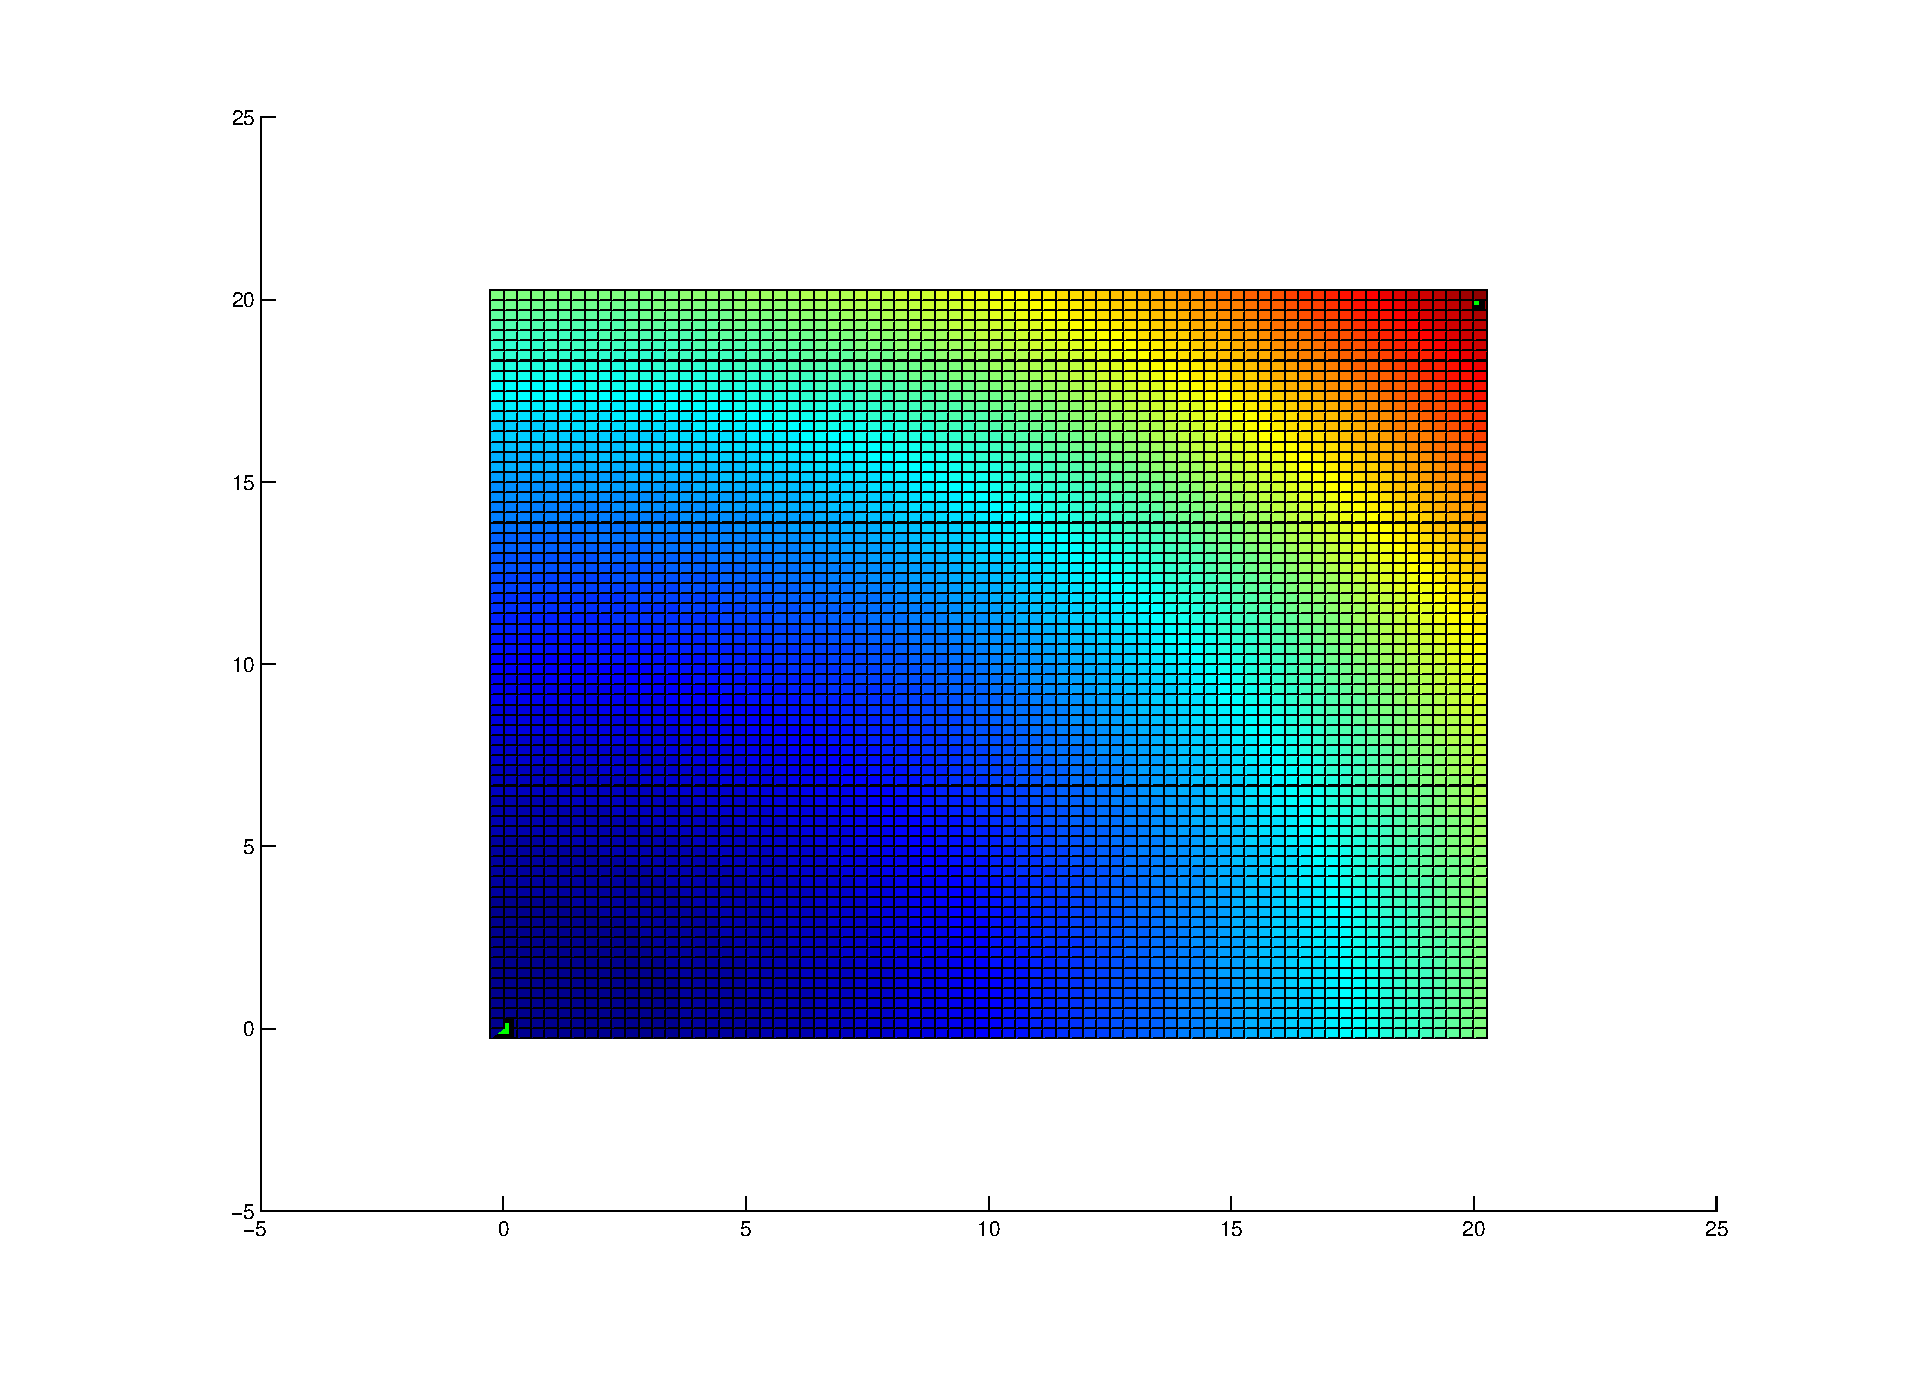
\includegraphics[width=0.5\linewidth]{f2_xy}
 }
 \subfigure[Widok Y-Z]{
  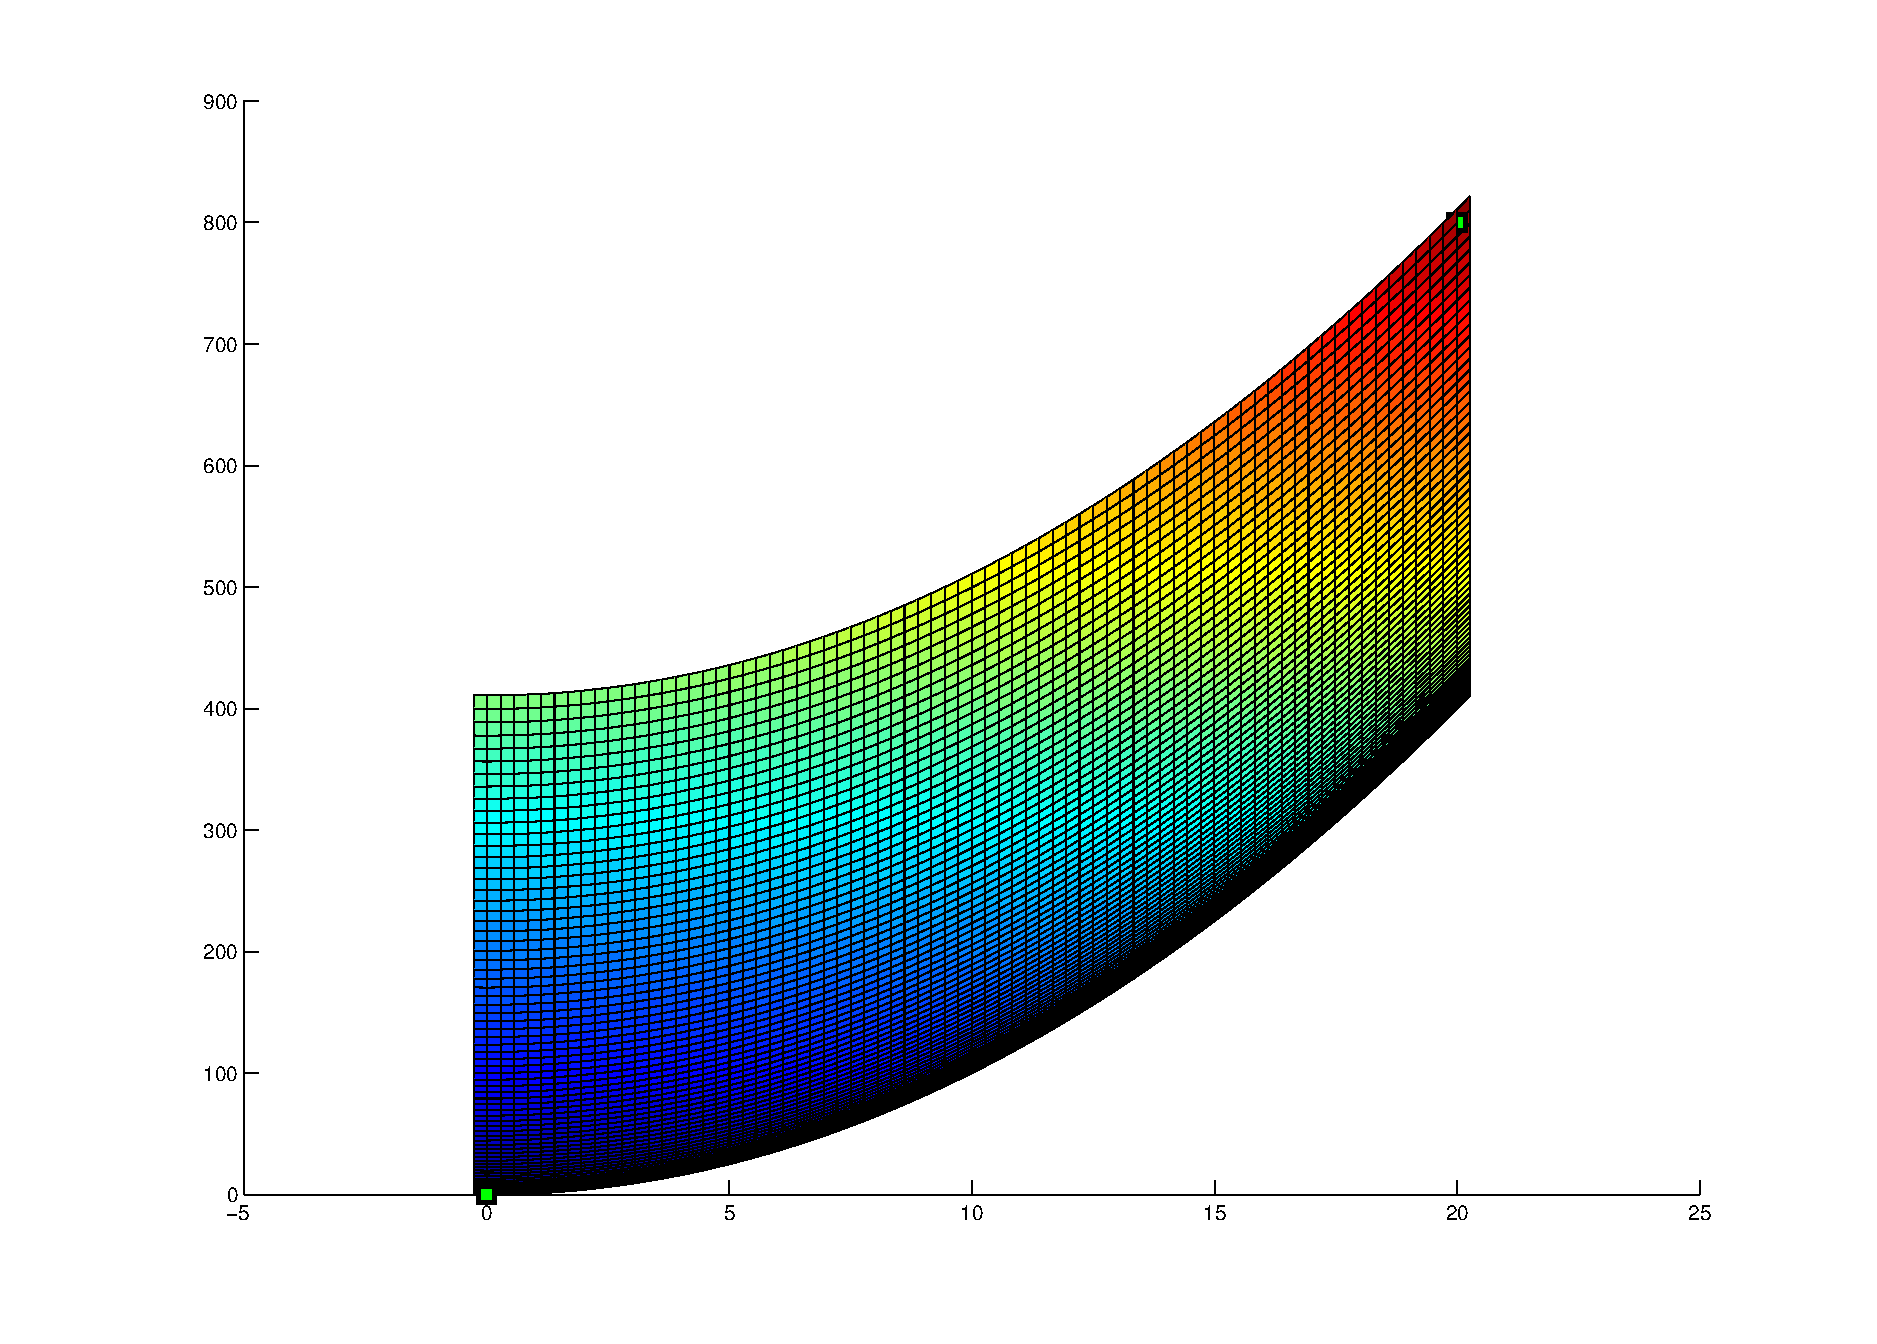
\includegraphics[width=0.5\linewidth]{f2_yz}
 }
}
\caption{Wyniki funkcji 2.}
\end{figure}

\subsection{Funkcja testowa 2}
Wykorzystaliśmy funkcję
\begin{equation}
  z = x^2 + y^2
\end{equation}

Punkt startowy: $(20, 20)$.

Rozwiązanie znalezione przez WolframAlpha\footnote{\url{http://www.wolframalpha.com/input/?i=min\%28x^2+\%2B+y^2\%29}}: $(0, 0)$, rozwiązanie znalezione programem (2 iteracje): $(0, 0)$.

\begin{figure}
\noindent\makebox[\textwidth]{%
 \subfigure[Widok X-Y]{
  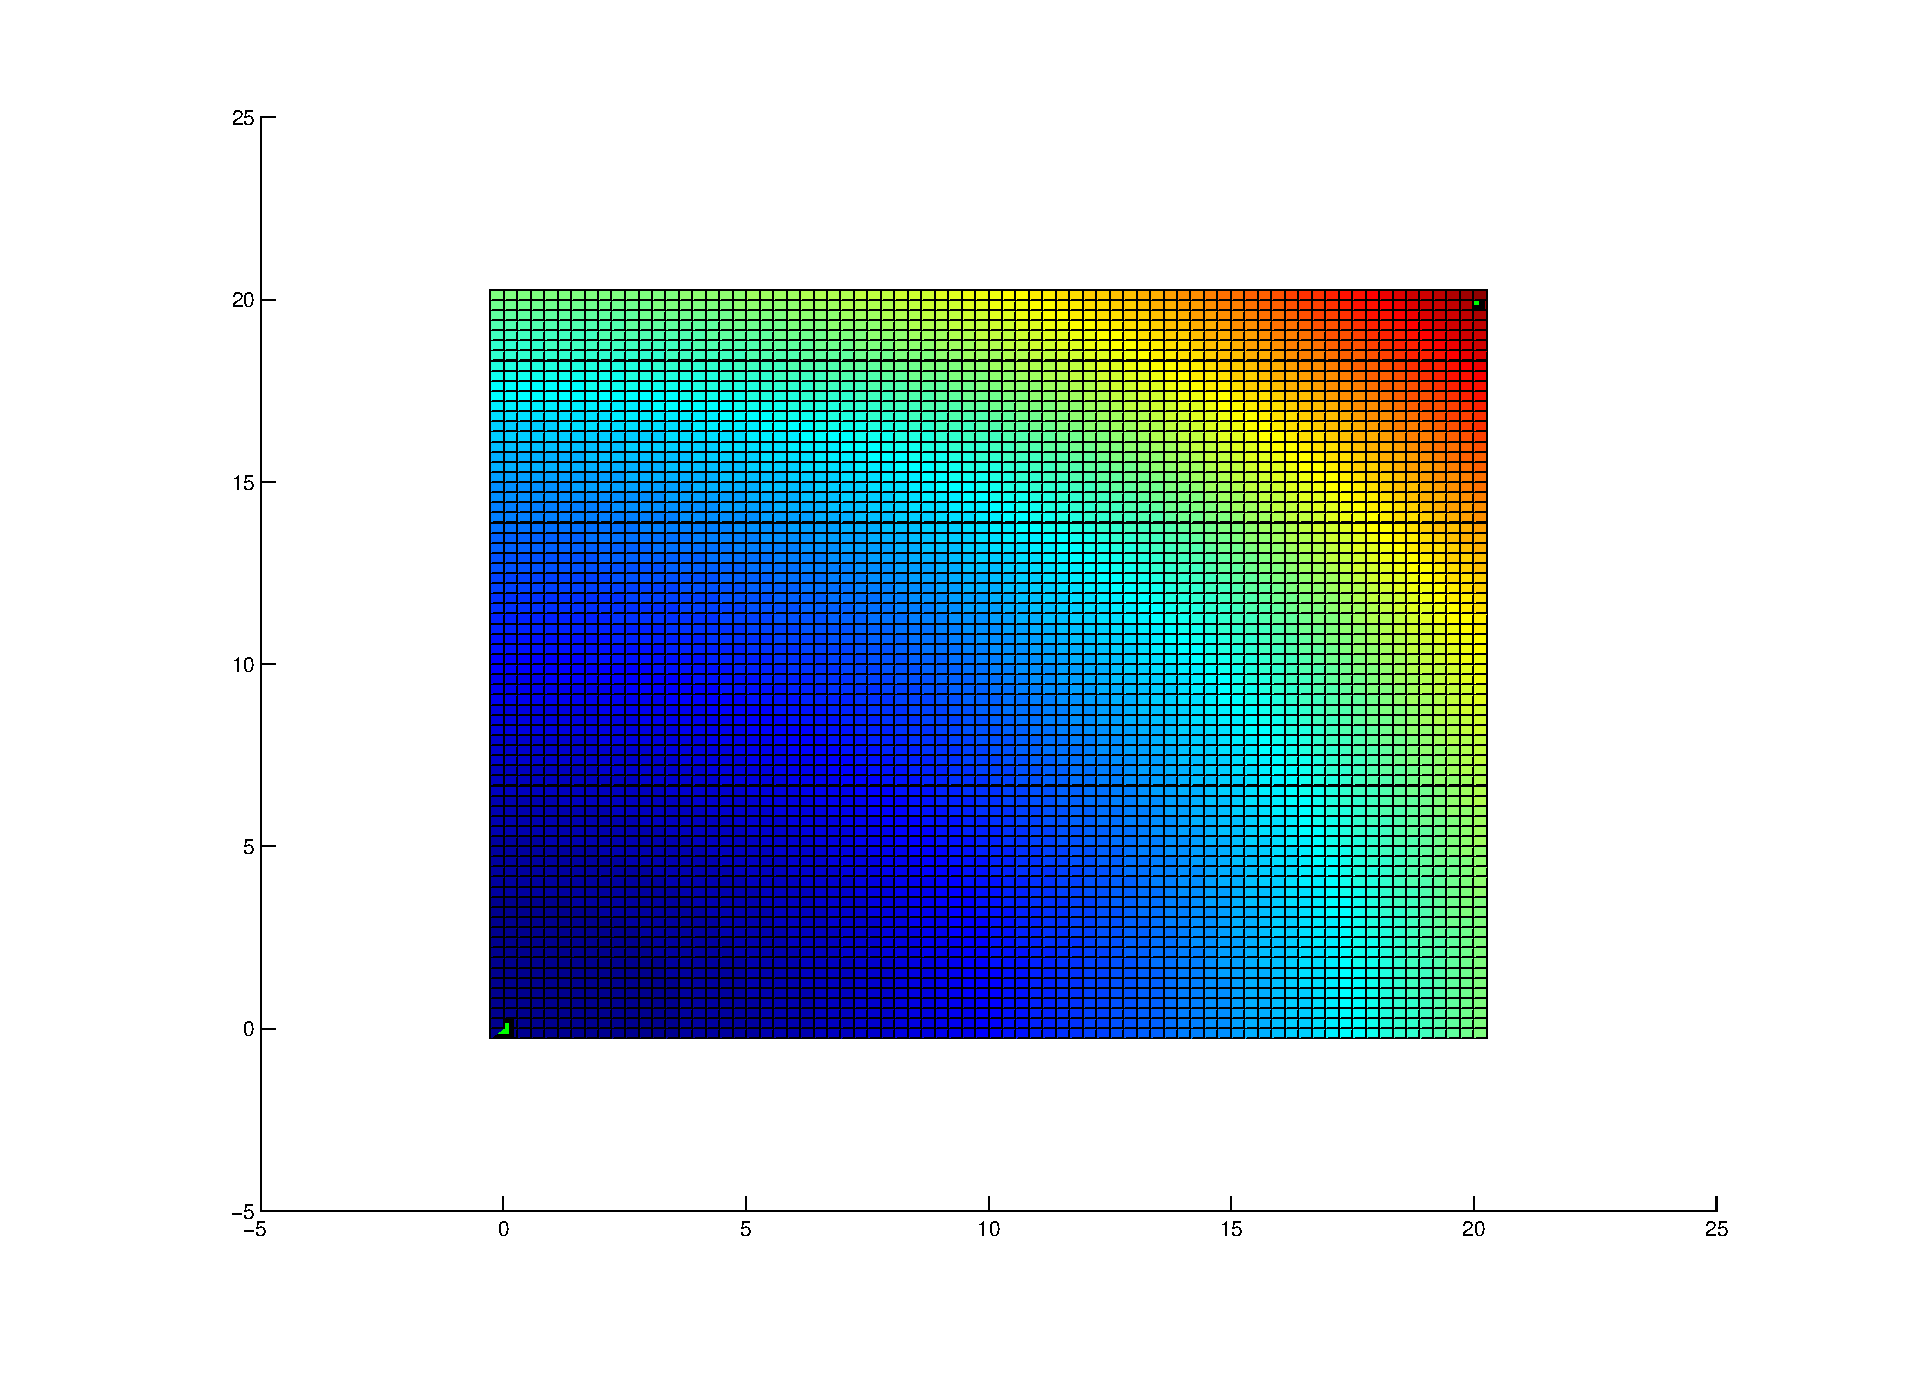
\includegraphics[width=0.5\linewidth]{f2_xy}
 }
 \subfigure[Widok Y-Z]{
  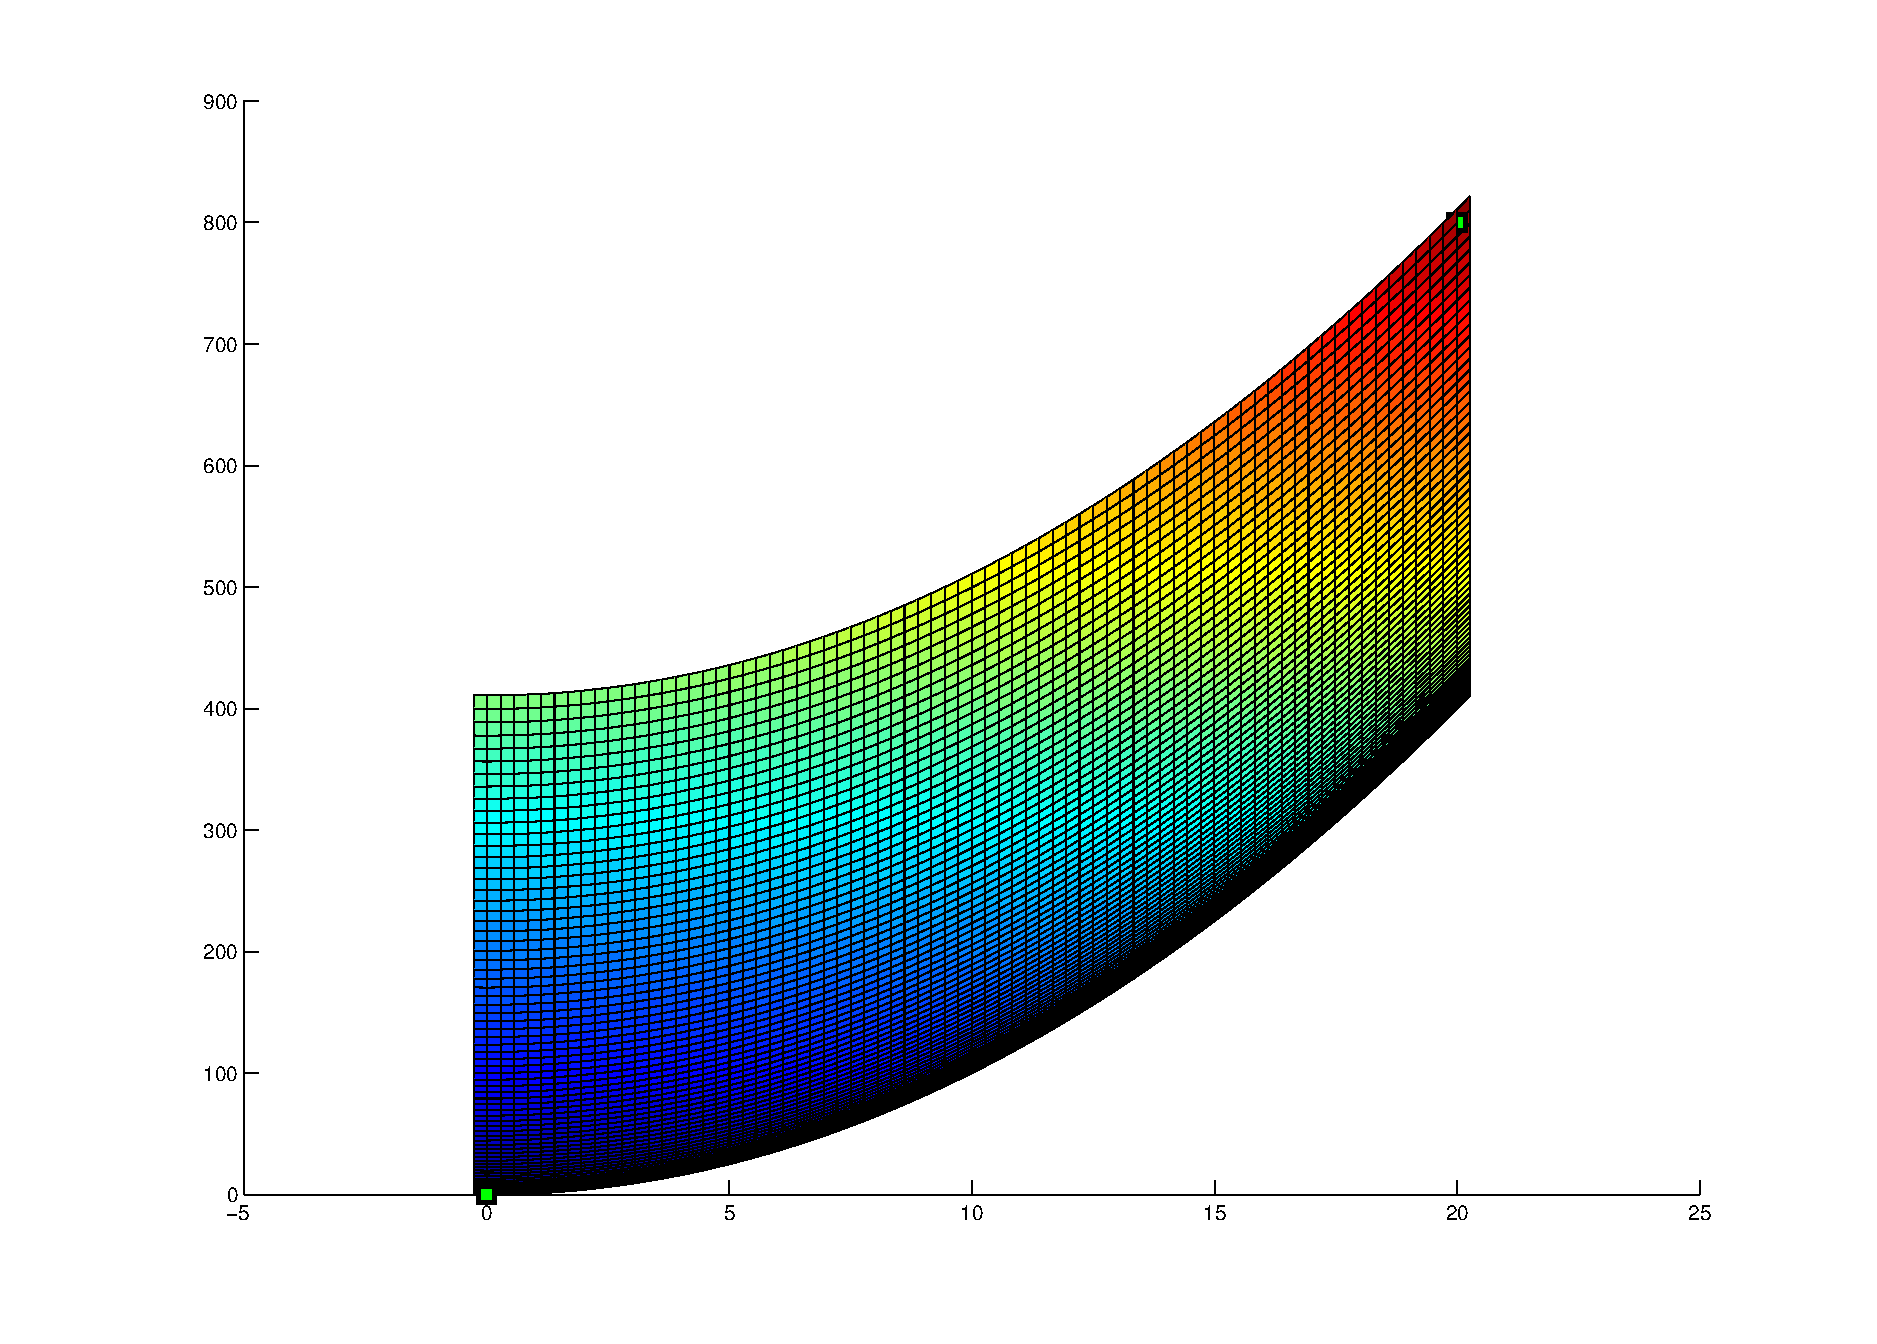
\includegraphics[width=0.5\linewidth]{f2_yz}
 }
}
\caption{Wyniki funkcji 2.}
\end{figure}

\section{Wnioski}

\begin{thebibliography}{99}
\bibitem{grega.wyklad}
Grega, Wojciech. \textit{Metody optymalizacji. Wykład 4} [online]. [dostęp: 27
marca 2011]. Dostępny w Internecie:
\url{http://aq.ia.agh.edu.pl/Aquarium/Dydaktyk/Wyklady/MO/2005-06/Wyklad04.PDF}
\end{thebibliography}

\end{document}
